\begin{figure}[H]
  \centering
  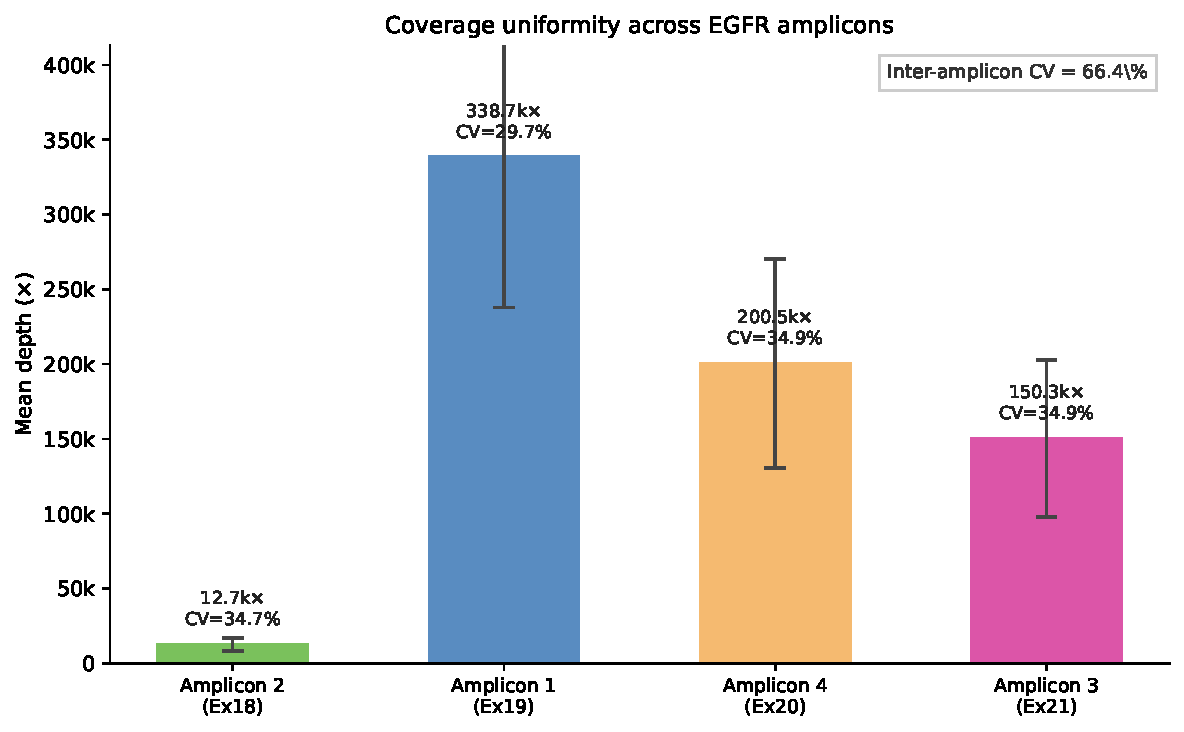
\includegraphics[width=0.85\textwidth]{figures/coverage_uniformity_plot.pdf}
  \caption{%
    Mean sequencing depth across the four EGFR amplicons.
    Each bar shows the mean per-base depth for one amplicon; error bars indicate
    $\pm$1 standard deviation.
    The within-amplicon coefficient of variation (CV) is annotated above each bar.
    The inter-amplicon CV is 66.4\%, reflecting the pronounced depth imbalance
    driven by Amplicon~2 (Exon~18, 12{,}650$\times$) relative to
    Amplicons~1, 3, and~4 (338{,}664$\times$, 150{,}290$\times$, and 200{,}484$\times$,
    respectively).
    Generated by \texttt{coverage\_uniformity\_plot.py} via Snakemake rule
    \texttt{coverage\_uniformity\_plot}.
  }
  \label{fig:coverage-uniformity}
\end{figure}
